\paragraph{Signatures including a Z boson}

\subparagraph{Mono-Z (leptonic) signature}

Acceptances for the mass and \tanb scans are shown in \autoref{fig:monoz_ll_acceptance} and \autoref{fig:monoz_ll_tanbma_acceptance}.  
In the mass scan, for points where the Jacobian peak is below the analysis's \MET cut, from $\ma = 100$ $\mA = 200$ to $\ma = 300$ $\mA = 400$, 
acceptance drops sharply approaching zero.  Above this region, acceptance levels are grouped into bands for fixed values of $\mA-\ma$. 
With increasing $\mA-\ma$ acceptances increases, gradually plateauing to a maximum value of 50\%.  In the inverted mass region, 
acceptances are generally lower than the rest of the mass scan, but for light values of \ma can reach values as large as 30\%.
In the \tanb scan, acceptances are largely independent of \tanb and constant for equal values of \ma.  For small values of \tanb and
$\ma < 350$ \GeV  there is slight drop in the acceptance caused by the softer \MET distribution from non-resonant decays. The event yield after the selection is shown in \autoref{fig:monoz_ll_tanbma_yield}.  

\begin{figure}
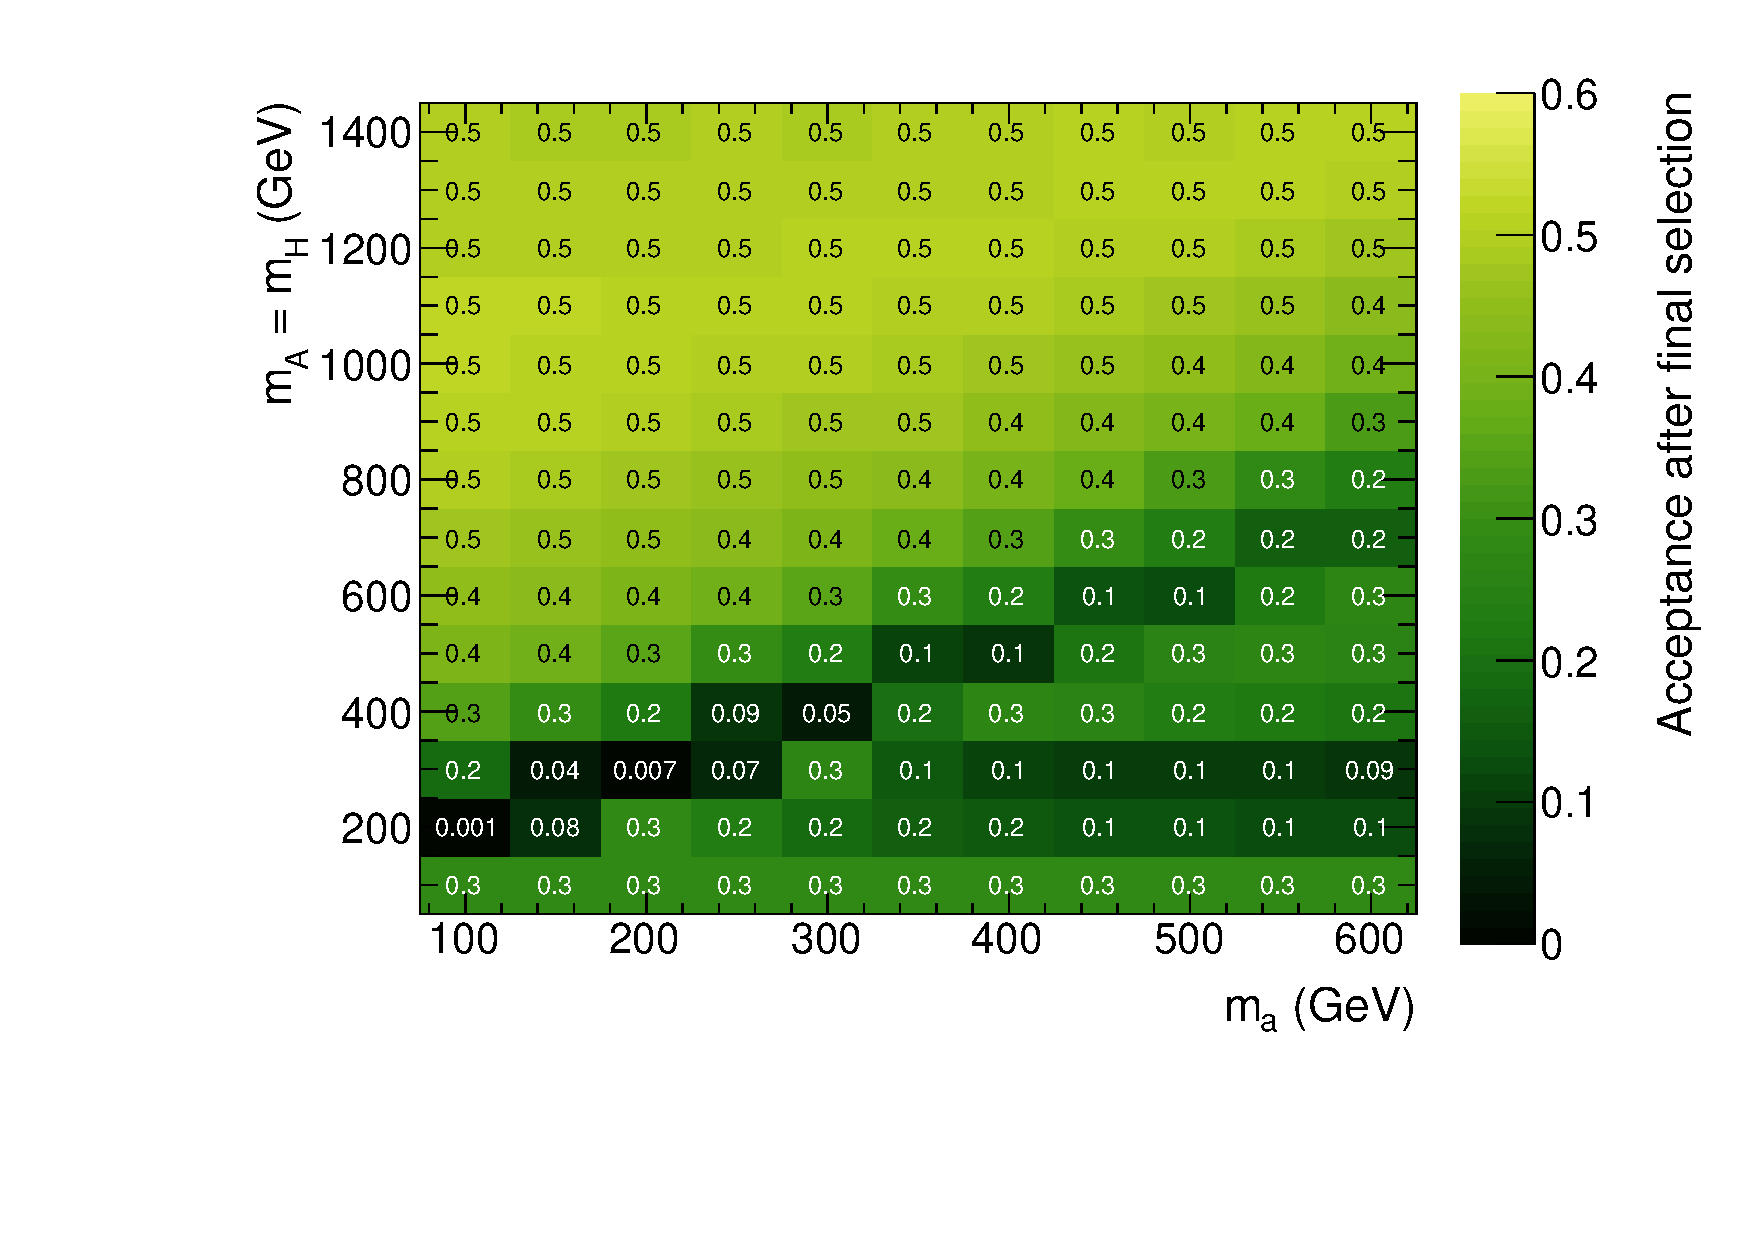
\includegraphics[width=\textwidth]{texinputs/04_grid/figures/monoz/leptonic/acceptance_dmwg-final_26300.pdf}
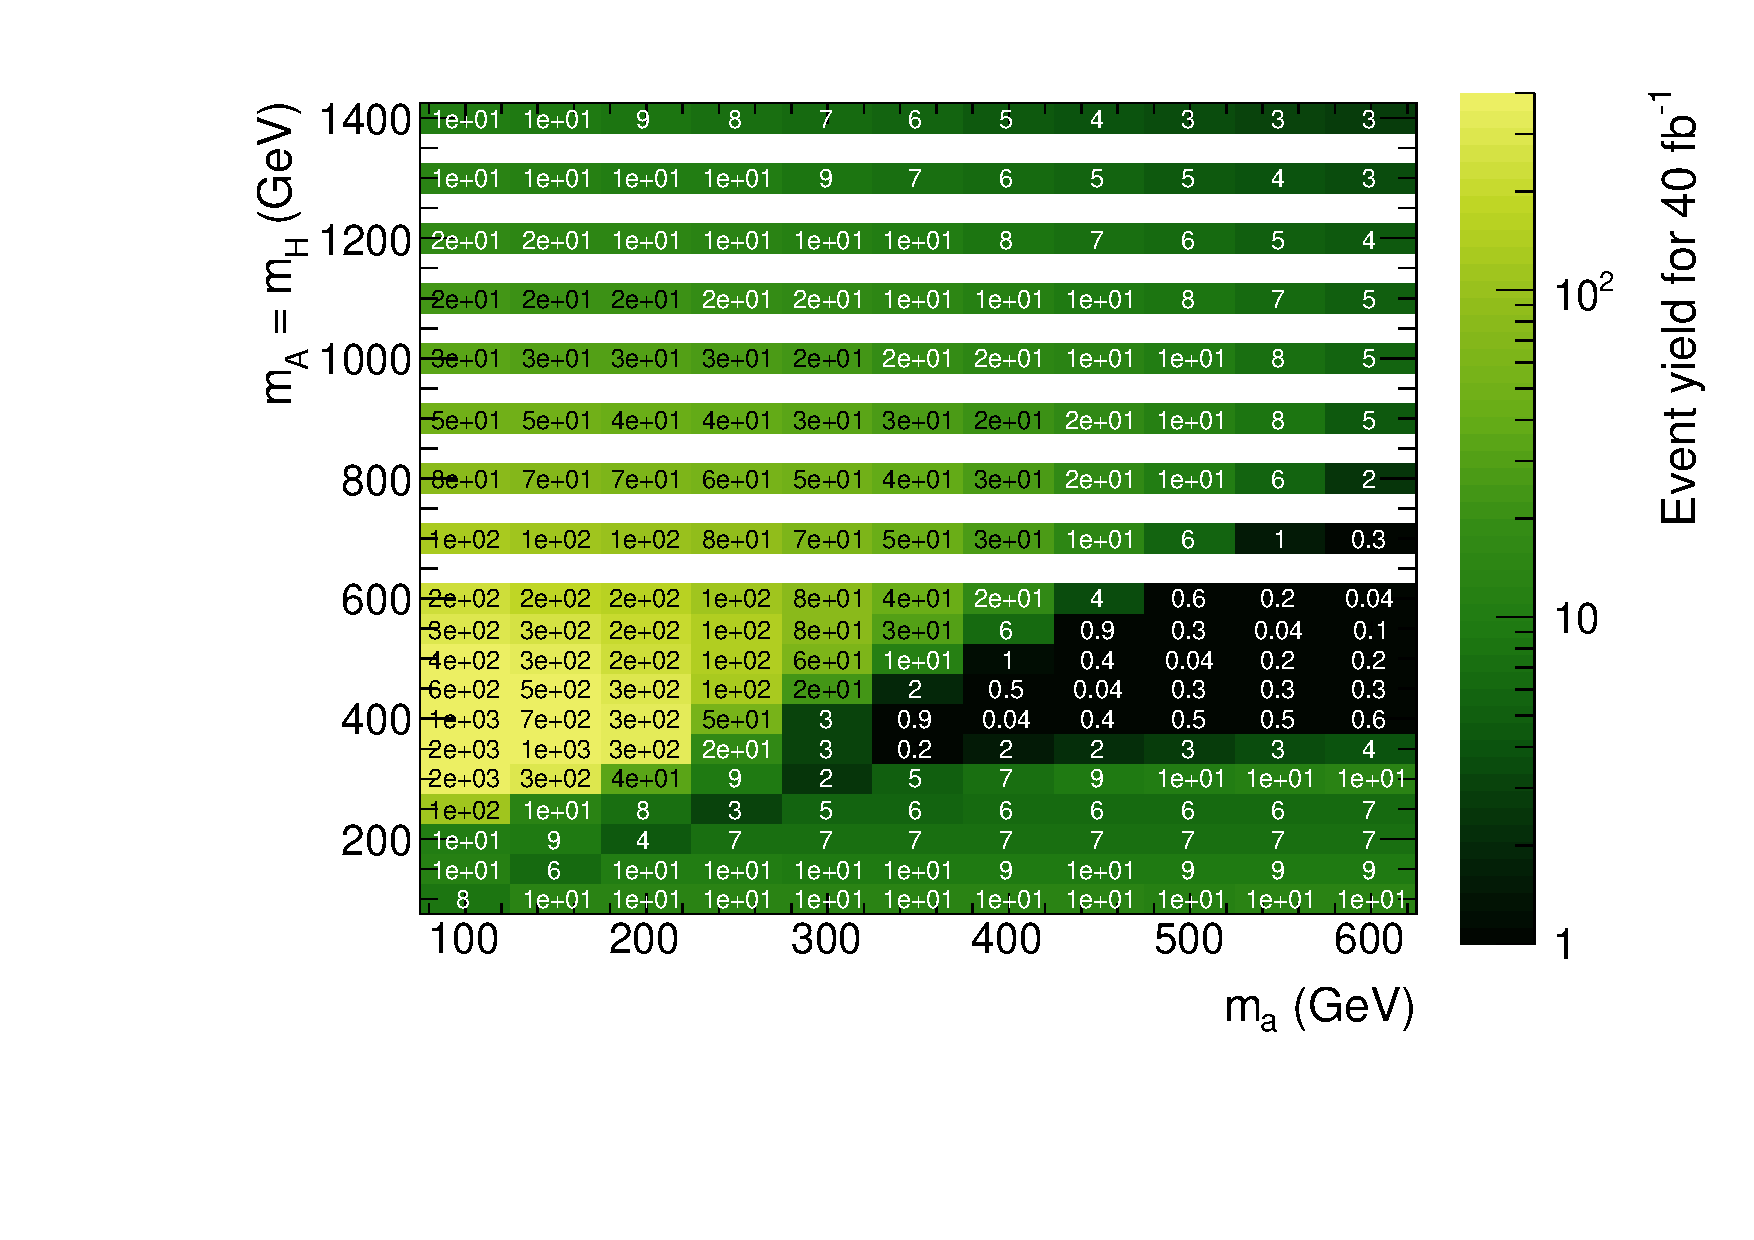
\includegraphics[width=\textwidth]{texinputs/04_grid/figures/monoz/leptonic/xs_2d_dmwg-final_26300_yield40fb.pdf}
\caption{Acceptance and event yields in the  \ma-\mA plane after applying the final selection. Event yields assume an integrated luminosity of $40~\ifb$. The acceptance is maximal for $\mA > \ma$, where it reaches 50 \%. In the inverted mass region $\mA < \ma$, lower values of 10-30\% are observed. In the intermediate region around $\mA \approx \ma + \mZ$, the acceptance is strongly suppressed as the a and Z bosons are produced approximately at rest.}
\label{fig:monoz_ll_acceptance}
\end{figure}

\begin{figure}
\centering
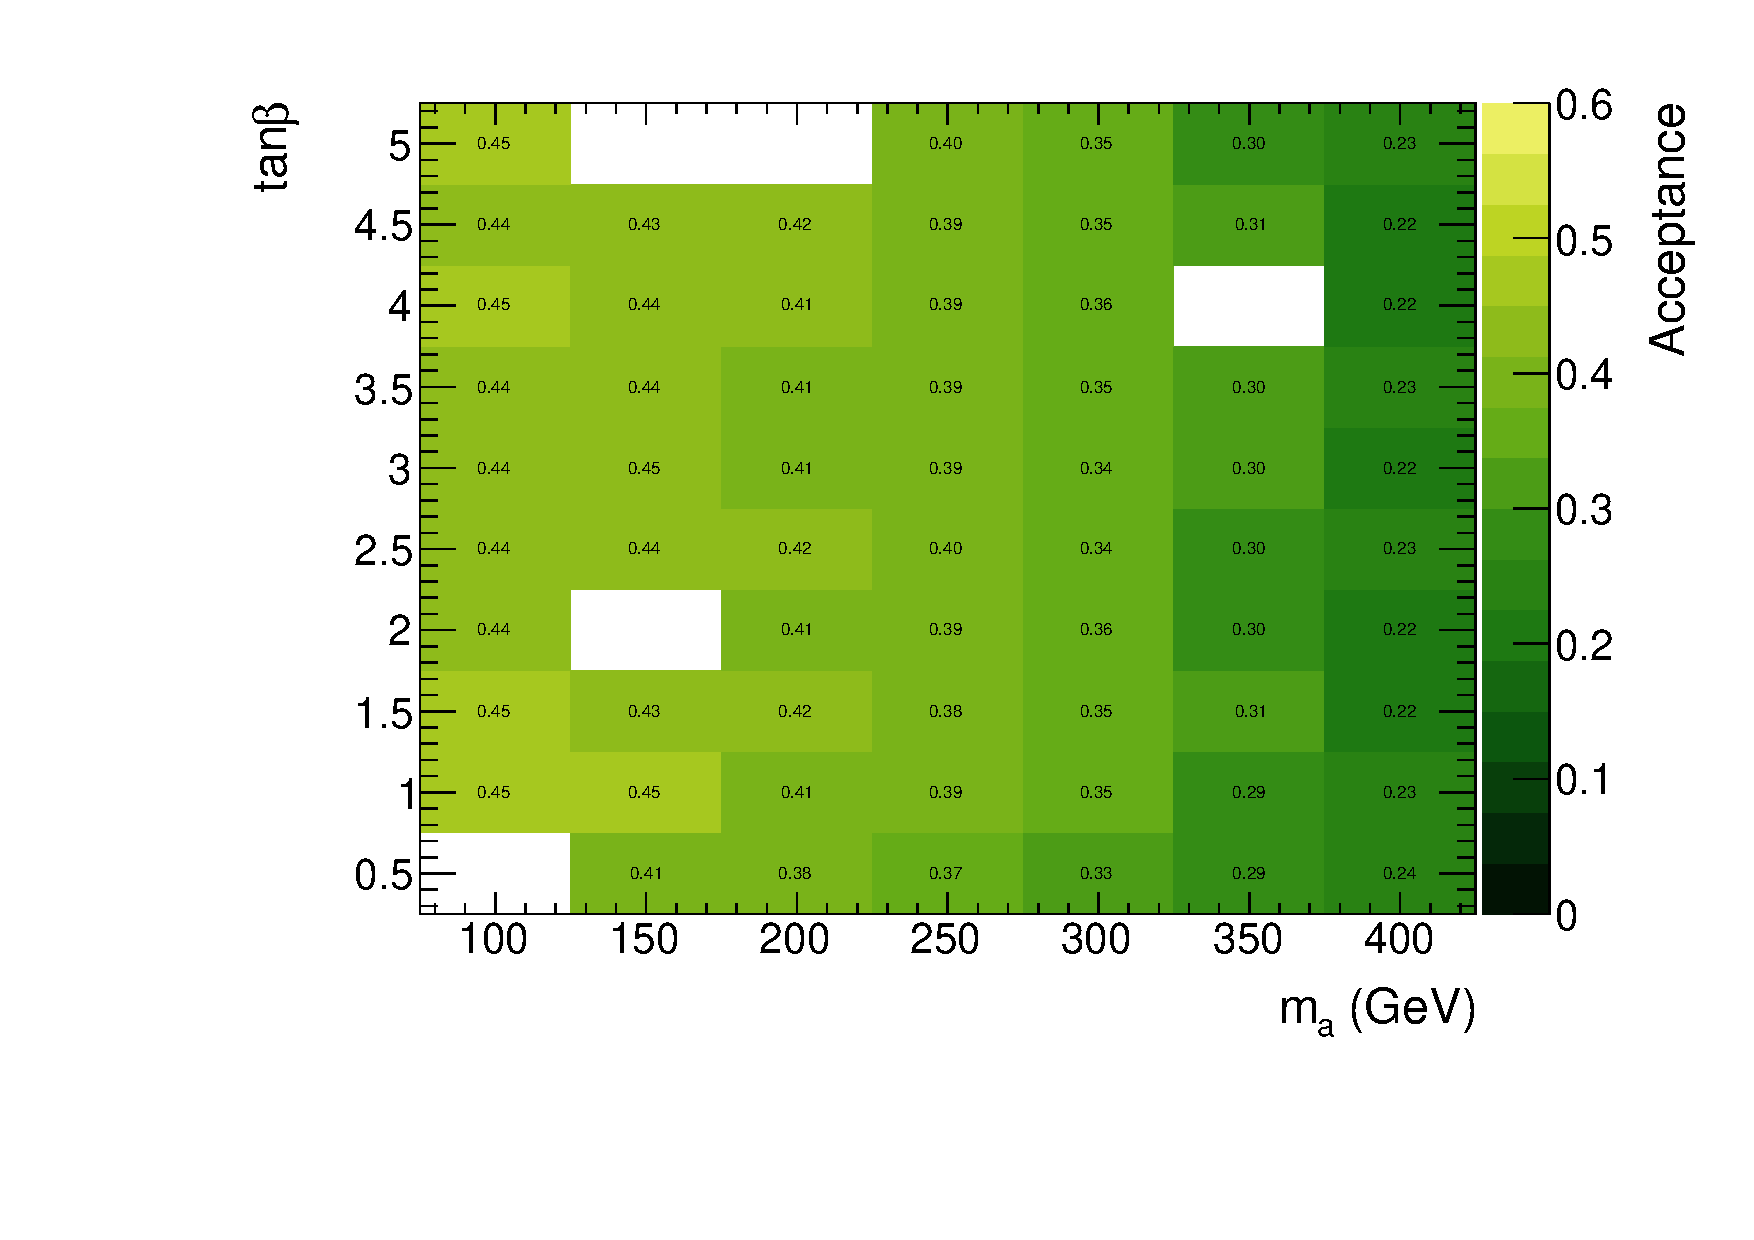
\includegraphics[width=0.6\textwidth]{texinputs/04_grid/figures/monoz/leptonic/tanbma_ae_ll.pdf}
\caption{Acceptances across the \ma-\tanb scan.  Acceptance is flat over \tanb for constant values of \ma.}
\label{fig:monoz_ll_tanbma_acceptance}
\end{figure}

\begin{figure}
\centering
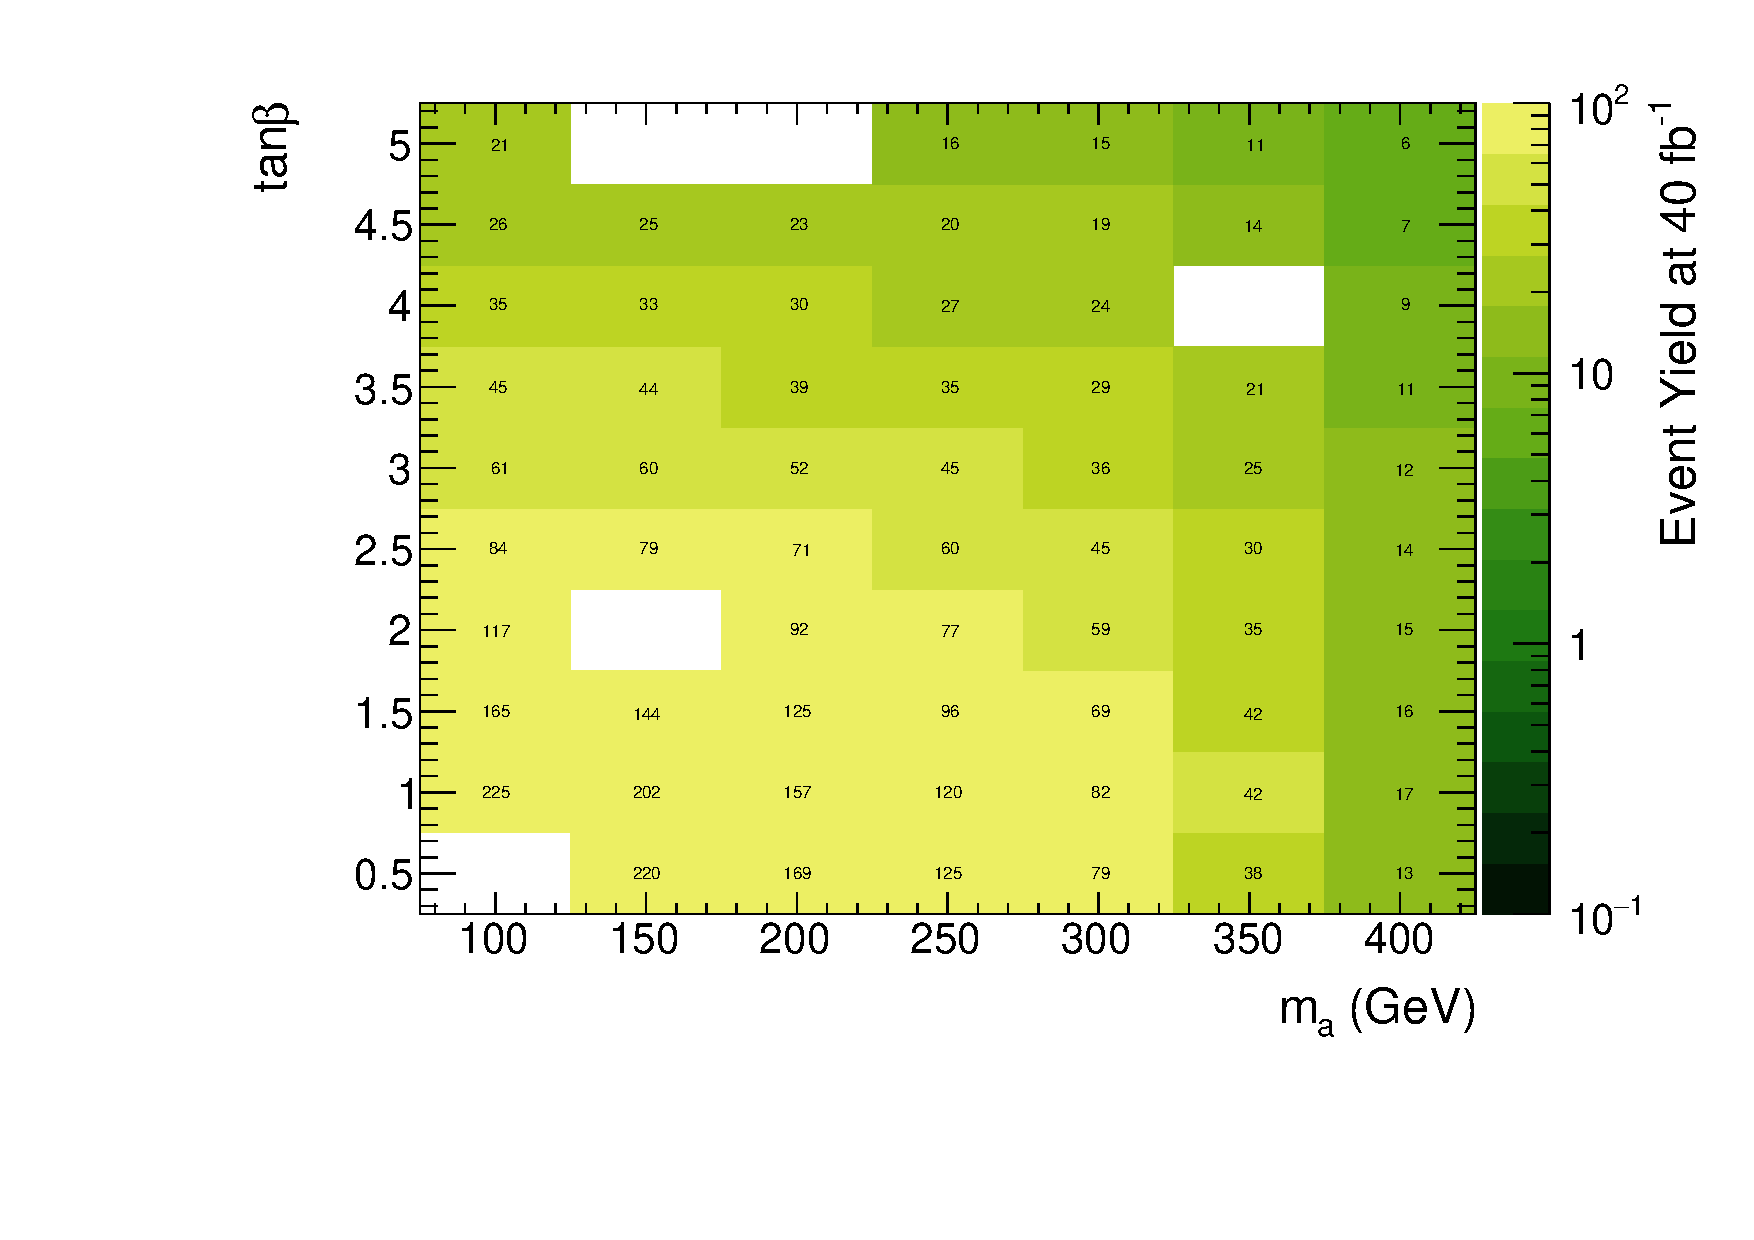
\includegraphics[width=0.6\textwidth]{texinputs/04_grid/figures/monoz/leptonic/tanbma_yield_ll.pdf}
\caption{Event yield in the \ma-tanBeta grid, for an integrated luminosity of $40~\ifb$.  The number of expected events diminshes with increasing tanBeta and \ma.  \mA fixed to 600 GeV and sinTheta to 0.35}
\label{fig:monoz_ll_tanbma_yield}
\end{figure}
